%!TEX root = or_benchmarks_paper.tex
\section{Multi-Period Newsvendor Problem with Lead Times}
\label{sec:newsvendor}

The Newsvendor problem (see e.g. \cite{zipkin2000foundations}) is a seminal problem in inventory management wherein we must decide on an ordering decision (how much of an item to purchase from a supplier) to cover a single period of uncertain demand. The objective is to trade-off the various costs incurred and revenues achieved during the period, usually consisting of sales revenue, purchasing and holding costs, loss of goodwill in the case of missed sales, and the terminal salvage value of unsold items.

In practice, decisions are rarely isolated to a single period, and they are repeatedly and periodically taken and thus have a downstream impact. This makes the problem non-trivial, as compared to the single-period Newsvendor which has a known solution when the demand distribution is known. Additionally, purchased units do not, in general, arrive quasi-instantaneously, but rather after a few periods of transit from the vendor to their final destination, known as the lead time. The presence of lead times further complicates the problem. The multi-period newsvendor problem with lead times under the lost-sales model, where customers leave if there is no stock to satisfy their demand, is known not to admit a simple solution such as an order-up-to policy (which maintains an inventory level, and orders up to that level whenever inventory levels fall).

% with a simple structure. Simple structures include an  as is the case in the absence of lead time or when a backlogging assumption is made.

Solving the multi-period newsvendor problem with lead times and lost sales is a notoriously difficult problem \citep{zipkin2008old}. It requires keeping track of orders placed in different periods, leading to what is known as the \emph{curse of dimensionality}, rendering any exact solution impractical even for small lead times of 2 and 3 periods, and outright infeasible at higher dimensions. As a result, the problem forms a good test-bed for RL algorithms given that the observation of rewards is delayed by the lead time and that it can be formulated as a Markov Decision Problem. Additionally, a number of heuristics have been developed for the lost sales problem, often based on order-up-to level policies for the equivalent model with backlogged demand. Comparisons in the performance of these two policies have been studied \cite{janakiraman2007comparison}, and it has been shown that order-up-to policies are asymptotically optimal and robust (in some sense) \cite{huh2009asymptotic,bijvank2014robustness}, thus making for good benchmark policies.

\subsection{Problem formulation}
We consider the stationary, single-product, multi-period dynamic inventory management problem with vendor lead time (VLT) and stochastic demand. Here, the VLT $l$  refers to the number of time steps between the placement  and receipt of an order. The demand $D$ is assumed to be stationary and Poisson distributed with mean $\mu$. Items are purchased at a cost $c$ and sold at a price $p$, and incur a penalty for lost sales $k$ for each unit of unmet demand while any unit left over at the end of a period incurs a holding cost $h$. A discount factor $\gamma$ is used.


The problem is formulated as a Markov Decision Process: 
\begin{description}[style=unboxed,leftmargin=0cm]
\item[State:] The state $S$ of the problem is given by
\begin{align*}
S=(p,c,h,k,\mu,x_0,\ldots,x_{l-1})
\end{align*}
where $x_0$ is the on-hand inventory, $x_1$ the units to be received one period hence, and so on.
\item[Action:] In each period the state of the system is observed and an action $A=q$ is taken, consisting of the size of the order placed and to arrive $l$ time periods later.
\item[Reward:] We first incur the purchasing cost corresponding to the procured units given the action $a$.
A realization $d$ of the demand $D$, which we recall is Poisson distributed with mean $\mu$, is then observed, and demand is satisfied as much as is possible given on-hand levels. Missed sales incur a loss of goodwill $k$ per unit, while leftover units incur a holding cost $h$:
\begin{align*}
R &= p\min(x_0,d) - c a - h (x_0 - d)^+ - k (d - x_0)^+.
\end{align*}
where $(x)^+=\max(x,0)$.
\item[Transition:] The state of the system $S$ is then updated to $S_+$ by moving all pipeline units downstream and incorporating the newly purchased units:
\begin{align*}
S_+ &= (p,c,h,k,\mu,(x_0 - d)^+ +x_1,x_2,\ldots,x_{l-1},a).
\end{align*}
\end{description}

\subsection{Related work}
Some recent work has started looking at the newsvendor problem using a data-centric approach \cite{rudin2014big} or a reinforcement learning approach \cite{oroojlooyjadid2016applying}. These have so far still remained focused on the single period problem and often trying to learn some of the inputs, such as demand. Few other papers have considered Reinforcement Learning in the context of inventory management, such as \cite{gijsbrechts2018can} where a dual sourcing problem is tackled using RL.

\subsection{Baseline solution} 

As noted in Section \ref{sec:newsvendor}, it is impractical or even infeasible to solve the problem exactly to get a baseline. However, it is possible to use heuristics that provide good approximations to the optimal solution. In particular, a way to tackle the problem is to approximate it by its backlogging counterpart, for which a closed form solution of the optimal policy exists in the form of an order-up-to policy characterized by the following critical ratio:
\begin{align*}
CR = \frac{p-\gamma c + k}{p-\gamma c + k + h}.
\end{align*}
As a result, letting $z^* = F_l^{-1}(CR)$, where $F_l$ is the cumulative distribution  function of the $l$ period demand, the policy is given by:
\begin{align*}
a&= \left(z^* - \sum_{i=0}^{l-1} x_i\right)^+.
\end{align*}


\subsection{RL solution} 


We used a Proximal Policy Optimization algorithms (PPO) \cite{schulman2017proximal} as implemented in the RLLib package \cite{liang2017rllib}, where the policy is represented by a neural network. We used a neural network of size (256,256) and the hyperparameters presented in Appendix \ref{appendix:newsvendor_hp}.


\subsection{Results}

We present the results obtained using a VLT of 5. The economic parameters were chosen so that $p,c\in[0,100]$, $h\in[0,5]$ and $k\in[0,10]$, while the demand mean $\mu$ was such that $\mu\in[0,200]$.

In the course of our experiments we saw that how we sampled the initial state and item characteristics is critical. We modified the sampling scheme so as to sample ``interesting" states and avoid trivial or misleading initial configurations. For example, it should be easily learned that nonprofitable items (including the penalty for lost sale) should not be purchased, but this is not really indicative of a good performance since in practice such items would not be part of inventory. Similarly, high initial inventory levels would not lead to any purchase either because inventory can simply be drained over long periods of time, resulting in a trivial decision that results in a high reward that would unfairly favor the perceived quality of the RL solution. 

As a result, the sampling was performed as follows: $p\sim U[0,100]$, $c\sim U[0,p]$, $h\sim U[0,\min(c, 5)]$, $k\sim U[0,10]$ and $\mu\sim U[0,200]$ for the economic and demand parameters; where $U[a,b]$ denotes a uniformly random variable between $a$ and $b$.  The initial state was simply set to be $\mathbf{0}$.
%The initial state was similarly sampled so as to be in a region where actions are meaningful: $x_0\sim U[0,l\mu]$ and $x_{i} \sim U[0,l\mu - \sum_{j=0}^{i-1} x_j]$ for $i=1,\ldots,l-1$; where $U[a,b]$ denotes a uniformly random variable between $a$ and $b$.

%Figure~\ref{fig:newsvendor_PPO} compares the results obtained by the RL algorithm to the baseline. As noted earlier, the results do not give full credit to the RL approach in part because its reward function incorporates a penalty term to guide the policies towards the feasible region, which artificially decreases its perceived performance. Ongoing experiments are more promising and will be reported on in future work.

Figure~\ref{fig:newsvendor_PPO} compares the results obtained by the RL algorithm to the baseline. We observe that the RL solution was nearing the benchmark when the experiment was stopped.


\begin{figure}
\centering
        %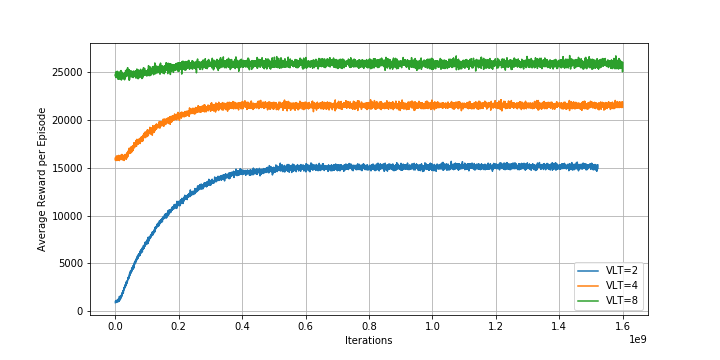
\includegraphics[width=0.5\textwidth]{images/newsvendor_PPO_big_minibatch_mlp_20_10.png}
        %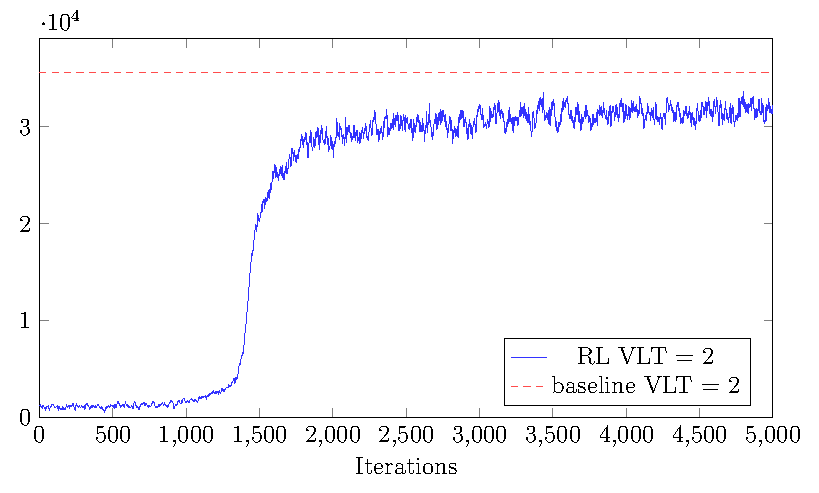
\includegraphics[width=0.45\textwidth]{images/newsvendor_l_2_ppo.pdf}
        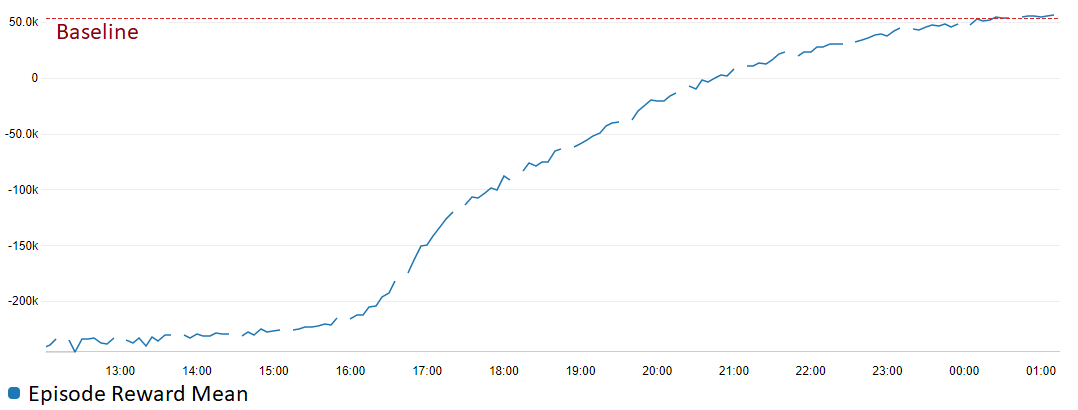
\includegraphics[width=0.45\textwidth]{images/newsvendor_edit.png}
    \caption{RL solution reward in the newsvendor problem.}
    \label{fig:newsvendor_PPO}
    	\vspace{-1em}
\end{figure}

While solving this problem numerically is intractable, the optimal inventory policy structures are well known. It is thus of interest to check whether their properties are being learned by the RL algorithm. Given the dimension of the problem, we cannot observe the entire policy, but can investigate slices thereof. We thus fix price, cost, holding cost, penalty for lost sale and mean demand to 50, 25, 0.5, 5 and 100, respectively, and plot the optimal policy in the space $(0,0,x_2,x_3,0)$ in Figure~\ref{fig:newsvendor_policy}. The figure shows contour curves of the buying quantity as a function of the inventory state. We observe that the algorithm is slowly learning the policy structure and we can start to observe monotonicity of the policy along most directions.

\begin{figure}[htbp]
\centering
        %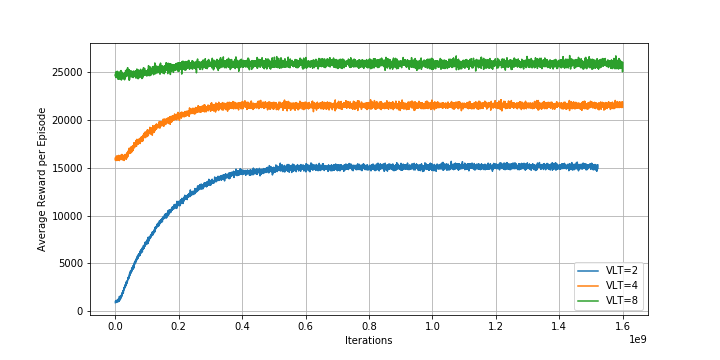
\includegraphics[width=0.5\textwidth]{images/newsvendor_PPO_big_minibatch_mlp_20_10.png}
        %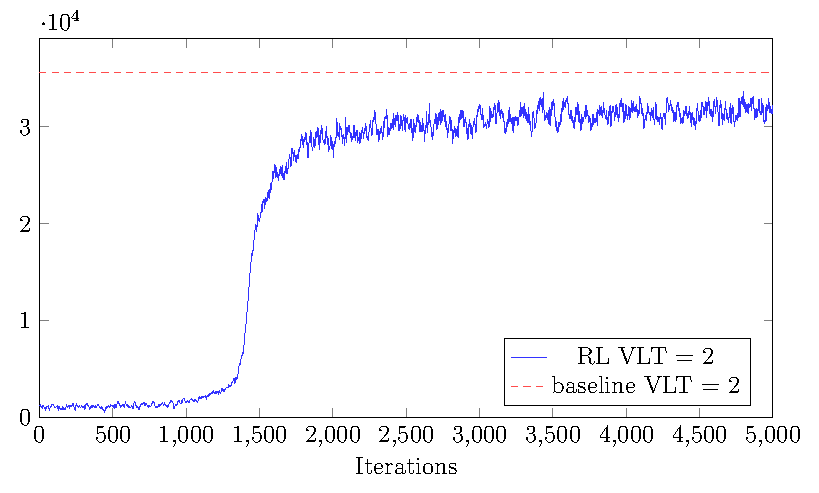
\includegraphics[width=0.45\textwidth]{images/newsvendor_l_2_ppo.pdf}
        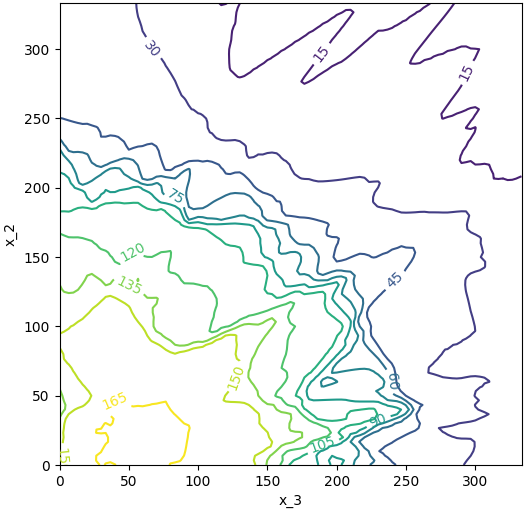
\includegraphics[width=0.4\textwidth]{images/newsvendor_policy.png}
    \caption{Slice of the learnt policy for the multi-period newsvendor.}
    \label{fig:newsvendor_policy}
    	\vspace{-1em}
\end{figure}
